\documentclass{scrartcl}

\usepackage{amsmath}
\usepackage{amssymb}
\usepackage{fancyhdr}
\usepackage{minted}
\usepackage{enumitem}
\usepackage{hyperref}
\usepackage{multirow}
\usepackage[table]{xcolor}
\usepackage{svg}
\usepackage{caption}
\usepackage{subcaption}
\usepackage{scalerel}
\usepackage{amsfonts}

\author{Jelmer Firet (s1023433, \href{mailto:jelmer.firet@ru.nl}{jelmer.firet@ru.nl}) \and
Bram Pulles (s1015194, \href{mailto:bram.pulles@ru.nl}{bram.pulles@ru.nl})}
\title{\textbf{Automated Reasoning\\Practical Assignment -- Part 2}}

\pagestyle{fancy}
\fancyhf{}
\fancyhead[L]{Automated Reasoning PA 2|Jelmer Firet \& Bram Pulles}
\fancyhead[R]{\thepage}

\setminted{autogobble,tabsize=4,fontsize=\scriptsize}
\setlength{\parindent}{0pt}

\newcommand{\black}{\cellcolor{black}\color{white}}

\begin{document}
\maketitle

\section{Groups} % (fold)
\label{sec:groups}
\begin{enumerate}[label=\alph*)]
\item
	We proved that $I*x=x$, $inv(inv(x))=x$ and $inv(x)*x=I$ by putting all of
	the given formulas \textit{literally} in prover9, see
	\texttt{groups\_a1.in}.

	Using mace4, we show that, in general, $inv(x*y)=inv(x)*inv(y)$ does not
	hold. The smallest group for which this does not hold has size $6$, see
	\texttt{groups\_a2.in} and appendix \ref{apx: groups}.
\item
	Using mace4, we show that the smallest non-Abelian group has size $6$,
	again by \textit{literally} putting in the formulas provided, see
	\texttt{groups\_b.in} and appendix \ref{apx: groups}.
\item
	We use the fact that $x^2 = x * x$, $x^3 = x * (x * x)$ and $x^4 = x * (x *
	(x * x))$ this makes encoding $x^n = I$ straightforward for $n = 2, 3, 4$.

	Using prover9, we show that for $n=2$ all such groups are Abelian, see \texttt{groups\_c1.in}.

	Using mace4, we show that for $n=3$ the group is not Abelian in general and
	the smallest counterexample has size $27$, see \texttt{groups\_c2.in}.

	Using mace4, we show that for $n=4$ the group is not Abelian and the
	smallest counterexample has size $8$, see \texttt{groups\_c3.in} and
	appendix \ref{apx: groups}.
\end{enumerate}
% section groups (end)

\pagebreak
\section{Robot} % (fold)
\label{sec:robot}

	\subsection{Explanation} % (fold)
	\label{sub:explanation}
	In this problem we are given a grid with colored cells. We should program a robot for this grid so that the robot will always find it's way to one of the goal cells if it starts on any start cell.
	The robot can detect the color of the cell it is on and decide based on that color which direction to move. Our program should find the best assignment of directions to colors. We will Z3 to find this assignment.

	In our program we read the grid from a csv file.
	We then determine the number of colors in this grid.
	For each color we make a Z3 integer that will store the direction to move for that color. The values of this integer correspond to the following directions:\\

	\begin{tabular}{l|ll}
		value & direction & effect on coordinates\\
		\hline
		0 & north & decreasing row\\
		1 & east & increasing column\\
		2 & south & increasing row\\
		3 & west & decreasing column\\
	\end{tabular}\\

	To ensure that Z3 only assigns one of these, we add the following constraint:
	$$\mathtt{\forall_{color}: 0 \le direction[color] < 4}$$

	Now we want to evaluate the performance of an assignment. For this we want to know for every cell if we reach a destination, and if so in how many steps. We will add a Z3 integer storing this distance for every cell. For now we will say that this integer has the value $\infty$ if it can not reach a destination cell.\\

	We then specify how the distances interact with the commands. We will start with the simple cases; the destination and the lava. For a destination cell we do not need to move to reach a destination cell, therefore we add the following constraint:
	$$\mathtt{\forall_{0\le r<R}\forall_{0\le c<C}\text{ if }grid[r][c]=DESTINATION: dist[r][c]=0}$$
	We do something similar for lava. From a lava cell we cannot reach a destination cell, so we add the following constraint:
	$$\mathtt{\forall_{0\le r<R}\forall_{0\le c<C}\text{ if }grid[r][c]=LAVA: dist[r][c]=\infty}$$

	Now we will specify what the robot does for regular cells. For convenience we have a function $\mathtt{next(r,c,direction,steps)}$ that give the position we go to when we take $\mathtt{steps}$ steps to $\mathtt{direction}$ from cell $(\mathtt{r},\mathtt{c})$. This function takes into account that the robot stops at the edges of the grid.
	\begin{align*}
		&\mathtt{\forall_{0\le r<R}\forall_{0\le c<C}\forall_{0\le dir<4}\text{ if }\neg special(grid[r][c]):}\\
		&\mathtt{direction[grid[r][c]]=dir \implies dist[r][c]=1+dist[nr][nc]}\\
		&\text{ where }
		\mathtt{(nr,nc) = next(r,c,dir,1)}
	\end{align*}
	Note that we consider $1+\infty=\infty$. When we give $\infty$ an actual value, we will have to specify this special case explicitly.

	We can now specify how the ice cells work. We want $\mathtt{dist[r][c]}$ to store the worst-case distance to a destination cell. We will have a similar condition to the one for the regular cells, but take the maximum of the cells where we can end up. This translates into the following constraint:
	\begin{align*}
		&\mathtt{\forall_{0\le r<R}\forall_{0\le c<C}\forall_{0\le dir<4}\text{ if } grid[r][c] = ICE:}\\
		&\mathtt{direction[grid[r][c]]=dir \implies dist[r][c]=1+\max(dist[nr][nc],dist[nr',nc'])}\\
		&\text{ where }
		\mathtt{(nr,nc) = next(r,c,dir,1) \text{ and } (nr',nc') = next(r,c,dir,2)}
	\end{align*}

	Now we are ready to specify what we want to achieve, we want an assignment of directions to colors that minimizes
	$$\mathtt{\max_{0\le r < R, 0\le c < C, grid[r][c]=START} dist[r][c]}$$
	We do this by adding a Z3 integer for this goal and ask the Z3 optimizer to minimize this variable. Then we add the following constraint:
	$$\mathtt{\forall_{0\le r<R}\forall_{0\le c<C}\text{ if }grid[r][c]=START: dist[r][c]\le goal}$$

	Now we can choose a value for $\infty$. We do not want the $\mathtt{dist[r][c]}$ of start cells to be infinite, but otherwise the value does not matter. Therefore we choose the value of $\infty$ to be $\mathtt{goal+1}$. Then in all of the previous constraints of the form $\mathtt{dist[r][c]=\ldots}$ we add the extra option that $\mathtt{dist[r][c]=goal+1}$. This allows Z3 to assign values to all distances even in the case of an infinite loop.
	% subsection explanation (end)

	\subsection{Results} % (fold)
	\label{sub:results}
	When we run our program on the demogrid, we find that the minimal solution uses 11 steps\footnote{The problem statement gives a "solution for 10 steps", but the image shows a solution with 11 steps}. The assignment of directions is visualized in figure \ref{robot-demogrid-solution}.

	On grid (a) our program finds that the minimal solution uses 14 steps. The
	assignment of directions is visualized in figure
	\ref{robot-grid-a-solution}. On grid (b) our program also finds a minimal
	solution of 14 steps, which is visualised in figure
	\ref{robot-grid-b-solution}. On grid (c) our program also finds a minimal
	solution of 18 steps, which is visualised in figure
	\ref{robot-grid-c-solution}.

	\begin{figure}
		\begin{subfigure}{0.5\textwidth}
			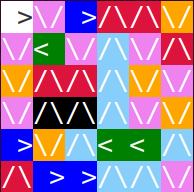
\includegraphics[width=0.9\textwidth]{resources/Screenshot from 2022-11-21 12-14-49.png}
			\caption{Solution for demo grid}
			\label{robot-demogrid-solution}
		\end{subfigure}
		\begin{subfigure}{0.5\textwidth}
			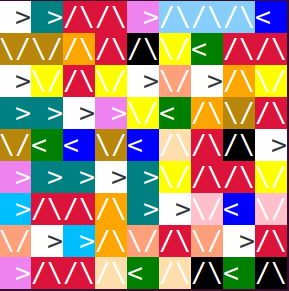
\includegraphics[width=0.9\textwidth]{resources/Screenshot from 2022-11-21 12-20-11.png}
			\caption{Solution for grid (a)}
			\label{robot-grid-a-solution}
		\end{subfigure}
		\begin{subfigure}{0.5\textwidth}
			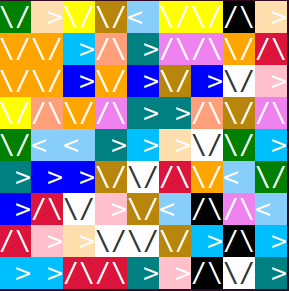
\includegraphics[width=0.9\textwidth]{resources/Screenshot from 2022-11-21 12-21-43.png}
			\caption{Solution for grid (b)}
			\label{robot-grid-b-solution}
		\end{subfigure}
		\begin{subfigure}{0.5\textwidth}
			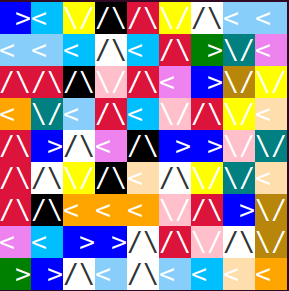
\includegraphics[width=0.9\textwidth]{resources/Screenshot from 2022-11-21 12-23-17.png}
			\caption{Solution for grid (c)}
			\label{robot-grid-c-solution}
		\end{subfigure}

	\end{figure}
	% subsection results (end)


\pagebreak
\section{Multiset Path Ordering}
\subsection{Explanation}
In this problem we are given a set of inequalities. These inequalities contain
terms which are either variables or functions over other terms. Our task is to
find a Multiset Path Ordering (MPO), which is an ordering on terms generated
from a total quasi-ordering relation $\trianglerighteq$ on the function
symbols, using multiset comparison.

To make our lives a bit easier we created a parser which can parse the
inequalities. To this end we created four data structures which can represent:
terms, functions, variables and inequalities. Notably, every one of these data
structures has a function \texttt{subterms} which recursively goes down the
term and gives all of its decendents. This is useful for when we define the
relations on terms.

We define the relations $\trianglerighteq, \rhd, \equiv$ on functions by
creating a new boolean variable for every relation and every pair of functions,
i.e. $\mathtt{\trianglerighteq_{fg}, \rhd_{fg}, \equiv_{fg}}$. To get the
correct behavior we add the constraints which define these relations, see
below. Note, that the relation $\leq$ is purely to prevent duplicates, such as
$\mathtt{f \trianglerighteq g \lor g \trianglerighteq f}$ \textit{and}
$\mathtt{g \trianglerighteq f \lor f \trianglerighteq g}$.

$$\mathtt{\forall_f \forall_{f \leq g} \trianglerighteq_{fg} \lor
\trianglerighteq_{gf}}$$

$$\mathtt{\forall_f \forall_{f \leq g} \equiv_{fg}\ =\ \trianglerighteq_{fg}
\land \trianglerighteq_{gf}}$$

$$\mathtt{\forall_f \trianglerighteq_{ff}}$$

$$\mathtt{\forall_f \forall_{g}\ \rhd_{fg} =\
\trianglerighteq_{fg} \land \neg \trianglerighteq_{gf}}$$

$$\mathtt{\forall_f \forall_{g} \forall_{h}\ \trianglerighteq_{fg} \land
\trianglerighteq_{gh} \to\ \trianglerighteq_{fh}}$$

We define the toprelations $\succsim, \succ, \approx$ on terms by creating a new
variable for every relation and every pair of terms, i.e. $\succsim_{st},
\succ_{st}, \approx_{st}$. To keep everything comprehensible we subdivide the
relations $\succ, \approx$ and create new variables $\succ_{a,st},
\succ_{b,st}, \succ_{c,st}, \approx_{a,st}, \approx_{b,st}$. The toprelations
are now defined using the constraints shown below.

$$\forall_s \forall_t \succsim_{st}\ =\ \succ_{st} \lor \approx_{st}$$
$$\forall_s \forall_t \succ_{st}\ =\ \succ_{a,st} \lor \succ_{b,st} \lor \succ_{c,st}$$
$$\forall_s \forall_t \approx_{st}\ =\ \approx_{a,st} \lor \approx_{b,st}$$

We define constraints for when the types do not match. For example, when
either $s$ or $t$ is a function we restrict $\neg\approx_{a,st}$. We do the
same for all the other subrelations, these constraints follow trivially and
will not be written out. The constraints for when the types do match are
nontrivial. The simple subrelation constraints are as follows.

$$\forall_{s = \mathtt{f}(s_1, \dots, s_n)} \forall_t \succ_{a,st}\ =
\bigvee_{s_i} \succsim_{s_i,t}$$

$$\forall_{s = \mathtt{f}(s_1, \dots, s_n)} \forall_{t = \mathtt{g}(t_1, \dots,
t_m)} \succ_{b,st}\ = \rhd_{\mathtt{f,g}} \land \bigwedge_{t_i} \succ_{s,t_i}$$

$$\forall_s \forall_t \approx_{a,st}\ =\ \approx_{st}$$

We are now left with the two constraints which use the multiset properties. We
will first take a look at $\approx_{b,st}$. Note, when $s$ or $t$ is not a
function, or the number of arguments in $s$ and $t$ are not the same we have
$\neg \approx_{b,st}$. For all of the other cases, where $s=\mathtt{f}(s_1,
\dots, t_n)$ and $t=\mathtt{g}(t_1, \dots, t_n)$, we check whether there exists
a permutation of the arguments of $t$ such that $\forall_n \approx_{s_i,t_i}$.
We define $\mathcal{P}(t_1, \dots, t_n)$ to give all the possible permutations
and use $t^p_i$ to denote $t_i$ in permutation $p \in \mathcal{P}$.

$$\forall_{s = \mathtt{f}(s_1, \dots, s_n)} \forall_{t = \mathtt{g}(t_1, \dots,
t_m)} \approx_{b,st}\ =\ \equiv_{\mathtt{f,g}} \land \bigvee_{p \in
\mathcal{P}(t_1, \dots, t_n)} \bigwedge_i \approx_{s_i,t^p_i}$$

The final constraint $\succ_{c,st}$ is the most elaborate of all. We use the
tip provided in the assignment. We generate all the possible $\mathtt{EQ}$ and
$\varphi$, such that $\exists_{i \in \{1, \dots, n\}}\ \mathtt{EQ}(i) = \bot$
and $\forall_i\ \mathtt{EQ}(\varphi(i)) = \top \to \forall_{j \neq i}\
\varphi(i) \neq \varphi(j)$. We can do this by generating all $\mathtt{EQ}$ and
$\varphi$, then filtering out the functions which do not satisfy the given
constraints. We define $\mathcal{P}^\mathtt{EQ}_\varphi(n, m)$ to give all the
$\mathtt{EQ}, \varphi$ pairs which satisfy the given constraints. The final
constraint is given below, seperated for when $\mathtt{EQ}(\varphi(i)) = \bot$
or $\mathtt{EQ}(\varphi(i)) = \top$.

$$\forall_{s = \mathtt{f}(s_1, \dots, s_n)} \forall_{t = \mathtt{g}(t_1, \dots,
t_m)} \succ_{c,st}\ =\ \equiv_{\mathtt{f,g}} \land \bigvee_{\mathtt{EQ},
\varphi \in \mathcal{P}^\mathtt{EQ}_\varphi(n, m)}
\left(
	\bigwedge_{i,\mathtt{EQ}(\varphi(i)) = \bot} \succ_{s_{\varphi(i)},t_i}
	\bigwedge_{i,\mathtt{EQ}(\varphi(i)) = \top} \approx_{s_{\varphi(i)},t_i}
\right)
$$
\subsection{Results}
Running Z3 with all the constraints and variable definitions as given above
provides us with the following ordering: $\mathtt{a \rhd c \rhd f \rhd g \rhd b
\rhd h \rhd d }$. Finding another symbol ordering is rather easy, we just added
the constraint $\mathtt{\neg \rhd_{h,d}}$. This gives us a new symbol ordering:
$\mathtt{a \rhd c \rhd b \equiv f \rhd g \rhd d \rhd h}$.

The human-readable proof for the inequality
$\mathtt{h}(\mathtt{g}(x,\mathtt{g}(u,z)),\mathtt{c}(x,y,x,z)) \rhd
\mathtt{f}(\mathtt{d}(x,z),u)$ given the first ordering is as follows.
By 2b it suffices to proof that $\mathtt{h \rhd d}$ which holds, and
$\mathtt{h}(\mathtt{g}(x,\mathtt{g}(u,z)),\mathtt{c}(x,y,x,z))~\succ~x$, and
$\mathtt{h}(\mathtt{g}(x,\mathtt{g}(u,z)),\mathtt{c}(x,y,x,z))~\succ~z$. Now
these two inequalities trivially follow from recursively applying rule 2a until
a variable $x$ or $z$ is reached inside the arguments of $\mathtt{h}$, using 3a
on the variables completes the proof.

\pagebreak
\section{Mosaic} % (fold)
\label{sec:mosaic}
	\subsection{Puzzle} % (fold)
	\label{sub:puzzle}
	Our problem is to generate a minimal mosaic puzzle.
	Mosaic\footnote{Also known as: fill-a-pix} is a relatively simple puzzle.
	You are given a grid of squares in which some cells have a number.
	You should color each cell either white or black.
	A number indicates how many cells in the surrounding $3\times3$ should be colored black.
	Below you can find an example of a mosaic puzzle and its solution.

	\begin{figure}[H]
		\centering
		\includesvg[width=0.8\textwidth]{resources/mosaic}
	\end{figure}

	The puzzle we generate should satisfy the following requirements:
	\begin{enumerate}
		\item The puzzle has an unique solution.
		\item This solution should match the solution we provide as input.
		\item There are no other puzzles with the same solution that have fewer numbers given.
	\end{enumerate}

	We have made two programs to generate puzzles.
	The first uses a SMT solver iteratively to find constraints that are necessary for a puzzle to be unique. Then it runs another SMT solver to minimize the number of hints. The other approach uses the unsat core. While Z3 finds a small puzzle using this method, it is not guaranteed to satisfy (3).
	% subsection puzzle (end)

	\subsection{Generation using unsat core} % (fold)
	\label{sub:mosaic_unsat_core}
	Since we want to use the unsat core, we need to make a set of constraints that is not satisfiable. We will use this unsatisfiability to guarantee requirement (1), namely we will try to find a second solution.

	For this we add a variable for each cell, whether it is black in the second solution or not. Since we will be adding these later, we encode this as a 0-1 constrained Z3 integer:

	$$\forall_r,c:  0 \le \text{filled}_{r,c} \le 1$$

	Then we will add the constraint that at least one of those variable does not match the given solution (grid), so that we force Z3 to look for a second solution:

	$$\exists_{r,c}:  \text{filled}_{r,c} \ne \text{grid}_{r,c}$$

	We will ask Z3 to find this second solution to the puzzle with a number in every cell. Since we have a desired solution, we can determine which value the numbers should have. For every cell we add the constraint that it has the same number of black cells surrounding it in both solutions:

	$$\forall_{r,c}: \sum_{\substack{r-1\le r' \le r+1\\c-1\le c'\le c+1}}\text{grid}_{r',c'} = \sum_{\substack{r-1\le r' \le r+1\\c-1\le c'\le c+1}}\text{filled}_{r',c'}$$
	This formula does not handle the edges, but we do handle those cases in our code. Since we are interested in the positions of the numbers in the puzzle, we track these constraints so that Z3 will give them as part of the unsat core.

	Now that we have all constraints we ask Z3 to check if there is a solution.
	If there is a solution we print this alternate solution.
	There exist desired solutions for which this happens, but it is rare.

	Otherwise we ask Z3 for an unsat core. This gives us a list of the number constraints that guarantee there is no second solution. Since these constraints correspond with numbers in the grid, we have found a puzzle that satisfies requirements (1) and (2). We enabled the \texttt{core.minimize} flag of Z3 to try find a minimal puzzle. However the minimal unsat core of Z3 is "best-effort", and there is no guarantee that it is optimal. In particular, the example puzzle above has been generated with this program and has 15 numbers. However, our other program has found the following puzzle with 13 hints:

	\begin{figure}[H]
		\centering
		\includesvg[width=0.8\textwidth]{resources/mosaic-recursive}
	\end{figure}
	% subsection mosaic_unsat_core (end)

	\subsection{Generation using iteration} % (fold)
	\label{sub:mosaic_iteration}
	In this approach we use two Z3 optimizers.
	The first optimizer searches for constraints on where to place numbers and makes these constraints as small as possible.
	The second optimizer tries to find the smallest placement of numbers that satisfies the constraints generated by the first optimizer.\\

	The idea of the first optimizer that we try to find a puzzle that satisfies all the generated constraints but still has a different solution. Then we consider which hints can differentiate both solutions. These are exactly the cells where the count of surrounding black squares differ.
	Any puzzle with the desired solution as it's only solution must then have a number in at least one of those squares.\\

	The constraints we add to the first optimizer largely correspond with what we did for the unsat core. However, we now have three types of variables:

	\begin{tabular}{ll}
		hinted & a puzzle that satisfies the generated constraints\\
		filled & an alternate solution to that puzzle\\
		contributes & places where the count of surrounding black squares differ.
	\end{tabular}

	Again we encode these variables with a 0-1 constrained integer in Z3:

	$$\forall_{r,c}: 0\le \text{hinted}_{r,c} \le 1$$
	$$\forall_{r,c}: 0\le \text{filled}_{r,c} \le 1$$
	$$\forall_{r,c}: 0\le \text{contributes}_{r,c} \le 1$$

	We replace the number constraint with a new one that takes into account whether a number is placed into a cell:

	$$\forall_{r,c}: \text{hinted}_{r,c}\to\sum_{\substack{r-1\le r' \le r+1\\c-1\le c'\le c+1}}\text{grid}_{r',c'} = \sum_{\substack{r-1\le r' \le r+1\\c-1\le c'\le c+1}}\text{filled}_{r',c'}$$

	As before we require that the alternate solution differs in at least one cell from the desired solution:

	$$\exists_{r,c}:  \text{filled}_{r,c} \ne \text{grid}_{r,c}$$

	Next we encode that a cell differentiates both solutions when the black counts differ:

	$$\forall_{r,c}: \sum_{\substack{r-1\le r' \le r+1\\c-1\le c'\le c+1}}\text{grid}_{r',c'} = \sum_{\substack{r-1\le r' \le r+1\\c-1\le c'\le c+1}}\text{filled}_{r',c'}\to \text{contributes}_{r,c}=1$$

	The clause we generate has a literal for every cell that distinguishes both solutions. Since SMT solvers are generally faster on smaller clauses, we minimize the number of cells that distinguish both solutions.

	$$\sum_{r,c}\text{constributes}_{r,c} = \min_{}(\sum_{r,c}\text{contributes}_{r,c}
	)$$

	When we run the first optimizer, we can have two results.
	If the solver returns unsat, there is no puzzle that satisfies all generated constraints and has multiple solutions. In other words, all puzzles satisfying the generated constraints have a unique solution. We then use the second optimizer to find the smallest puzzle satisfying all generated constraints.\\

	In the other case the solver provides a model that includes a puzzle, an alternate solution and the places where the black counts differ. We will add a new clause to both optimizers that encodes that a puzzle should distinguish both solutions:

	$$\exists_{r,c : \text{model}(\text{contributes}_{r,c})=1}: \text{hinted}_{r,c}$$

	After adding this constraint we run the first optimizer again to see if there are still alternate solutions.\\

	The second optimizer is a lot easier.
	It only uses the hinted variables, and the constraint that these are 0 or 1.
	It also includes all generated constraints to guarantee that the resulting puzzle has an unique solution.
	Finally it has the goal to minimize the number of cells that are hinted.\\

	This optimizer will always give a model\footnote{Except in the rare cases where even the puzzle with a number in every cell has multiple solutions}.
	This model corresponds to a minimal puzzle with a unique solution. Suppose there is another puzzle that has fewer hints. Then this puzzle does not satisfy at least one of the generated constraints. But then the alternate solution we found in the step that generated this constraint is also an alternate solution to the puzzle. Therefore there are no smaller puzzles with a unique solution.
	% subsection mosaic_iteration (end)

	\subsection{Results} % (fold)
	\label{sub:results}
	We have discussed two approaches to generating minimal mosaic puzzles for a given solution.
	The unsat-core approach is more efficient since it uses features of Z3 directly. We were able to generate puzzles with a $20\times20$ grid within a couple of seconds. Unfortunately there is no guarantee that the generated puzzle is minimal, as we have shown with the example above.\\

	The iterative approach is quite slow. It took multiple minutes to find the puzzle that disproved minimality of the unsat-core puzzle. The largest puzzle we have been able to generate is $8\times 8$, and took a couple of hours of computation. We are however confident that it generates globally minimal puzzles. An added benefit of this approach is that it defines the space of unique puzzles, so we can easily adapt the goal to find unique puzzles with some other property. For example, we can look for a minimal puzzle that has no adjacent hints, something we cannot encode in the unsat-core approach.
	% subsection results (end)

% section mosaïc (end)

\appendix
\pagebreak
\section{Groups}
\label{apx: groups}
\begin{enumerate}[label=\alph*)]
	\item
		Smallest finite group for which $inv(x*y)=inv(x)*inv(y)$ does not hold.
		\begin{verbatim}
		interpretation( 6, [number=1, seconds=0], [

		    function(I, [ 0 ]),

		    function(c1, [ 1 ]),

		    function(c2, [ 2 ]),

		    function(inv(_), [ 0, 1, 2, 4, 3, 5 ]),

		    function(*(_,_), [
		        0, 1, 2, 3, 4, 5,
		        1, 0, 3, 2, 5, 4,
		        2, 4, 0, 5, 1, 3,
		        3, 5, 1, 4, 0, 2,
		        4, 2, 5, 0, 3, 1,
		        5, 3, 4, 1, 2, 0 ])
		]).
		\end{verbatim}

	\item
		Smallest non-abelian group.
		\begin{verbatim}
		interpretation( 6, [number=1, seconds=0], [

			    function(I, [ 0 ]),

			    function(c1, [ 1 ]),

			    function(c2, [ 2 ]),

			    function(inv(_), [ 0, 1, 2, 4, 3, 5 ]),

			    function(*(_,_), [
			        0, 1, 2, 3, 4, 5,
			        1, 0, 3, 2, 5, 4,
			        2, 4, 0, 5, 1, 3,
			        3, 5, 1, 4, 0, 2,
			        4, 2, 5, 0, 3, 1,
			        5, 3, 4, 1, 2, 0 ])
		]).
		\end{verbatim}

	\item
		\pagebreak
		Smallest non-abelian group with $x^4 = I$.
		\begin{verbatim}
		interpretation( 6, [number=1, seconds=0], [

			    function(I, [ 0 ]),

			    function(c1, [ 1 ]),

			    function(c2, [ 2 ]),

			    function(inv(_), [ 0, 1, 2, 4, 3, 5, 6, 7 ]),

			    function(*(_,_), [
			        0, 1, 2, 3, 4, 5, 6, 7,
			        1, 0, 3, 2, 5, 4, 7, 6,
			        2, 4, 0, 6, 1, 7, 3, 5,
			        3, 5, 1, 7, 0, 6, 2, 4,
			        4, 2, 6, 0, 7, 1, 5, 3,
			        5, 3, 7, 1, 6, 0, 4, 2,
			        6, 7, 4, 5, 2, 3, 0, 1,
			        7, 6, 5, 4, 3, 2, 1, 0 ])
		]).
		\end{verbatim}
\end{enumerate}

\end{document}
